% Thursday 26 Nov 2026 update: DLR wind atlas, drone energy model, first wind-aware planner.
% Build: sh DLR/slides/2026-11-26/build.sh  (numbers.tex is generated from the JSON results)
\documentclass[aspectratio=169,10pt]{beamer}
\usetheme{default}
\usecolortheme{dove}
\setbeamertemplate{navigation symbols}{}
\setbeamertemplate{footline}[frame number]
\usepackage[T1]{fontenc}
\usepackage[utf8]{inputenc}
\usepackage{lmodern}
\usepackage{amsmath}
\usepackage{booktabs}
\graphicspath{{../../atlas/results/}{../../planner/fig/}{../../meshStudy/report/fig/}}
\newcommand{\pic}[2]{\IfFileExists{../../atlas/results/#2}{\includegraphics[width=#1]{#2}}{%
  \IfFileExists{../../planner/fig/#2}{\includegraphics[width=#1]{#2}}{%
  \IfFileExists{../../meshStudy/report/fig/#2}{\includegraphics[width=#1]{#2}}{%
  \fbox{\parbox[c][2cm][c]{\dimexpr#1-2\fboxsep-2\fboxrule}{\centering\scriptsize\texttt{\detokenize{#2}}\\not generated yet}}}}}}
% generated by make_numbers.py
\newcommand{\NDirs}{12}
\newcommand{\ExtSentence}{The run with the worst drift (180$^\circ$) was continued by 200 iterations: the field changed by 0.2\,\% RMS of $U_\mathrm{ref}$ at 20\,m above ground.}
\newcommand{\MaxDriftPct}{0.41}
\newcommand{\FieldBlendMs}{131}
\newcommand{\QueryThousandMs}{1.3}
\newcommand{\SolveMinutes}{30--45}
\newcommand{\NLoo}{12}
\newcommand{\OscSentence}{Runs at 90$^\circ$, 120$^\circ$, 210$^\circ$, 330$^\circ$ oscillate by about 1\,\% of $U_\mathrm{ref}$ (limit cycle of steady RANS).}
\newcommand{\ReynoldsRmsTwenty}{0.4}
\newcommand{\ReynoldsRmsTen}{0.4}
\newcommand{\BlendSentence}{Rotate, then blend. At the real 30\,$^\circ$ spacing (255\,$^\circ$ from 240 and 270): 7.5\,\% RMS at 20\,m, 2.3\,\% at 40\,m. Plain linear blending: 8.3\,\% at 20\,m.}
\newcommand{\PlanNodes}{128\,232}
\newcommand{\NPairs}{40}
\newcommand{\PlanMapFile}{plan_map_240.png}
\newcommand{\PlanSentence}{40 random start--goal pairs ($\geq$\,250\,m apart, both legs), 12 wind directions. Shortest path (smoothed) vs.\ energy path (smoothed only where it lowers energy), both re-evaluated in the same wind. \textbf{Reading:} the wind-aware \emph{route} saves about 1\,\% at typical winds and 5\,\% at 8\,m/s (some trips 15--25\,\%). Flying at the right \emph{speed} is worth more (1--5\,\% from adapting it to the wind, 30\,\% from leaving 10\,m/s), and the \emph{direction} of a leg changes its cost by 30--62\,\% (A to B vs.\ back). So the cost function pays off mostly in speed scheduling and leg ordering; the route matters on windy days and in the shelter of buildings.}
\newcommand{\HoverW}{168.5}
\newcommand{\BestJm}{8.83}
\newcommand{\BestSpeed}{18.3}
\newcommand{\BuildStatus}{Built 25 Nov 2026 06:59 from 12 solved directions (+ validation runs: 240@10).}


\title{DLR campus: a wind atlas from \NDirs{} directions,\\and a first wind-aware path planner}
\author{Henry Delacroix}
\institute{Politecnico di Milano, Multidisciplinary Project SWARM-LINK (wind track)}
\date{26 November 2026}

\begin{document}

\begin{frame}
\titlepage
\begin{center}\scriptsize\textit{\BuildStatus}\end{center}
\end{frame}

% ---------------------------------------------------------------------------------------------
\begin{frame}{What was asked on 24 Nov, and what this deck covers}
\small
\textbf{Arthur's roadmap:} lookup table $\rightarrow$ cost function $\rightarrow$ trajectory planner
(shortest path vs.\ wind-aware) $\rightarrow$ drag and energy $\rightarrow$ RF term $\rightarrow$ RL with the cost as reward.

\medskip
\begin{columns}[T]
\begin{column}{0.5\textwidth}
\textbf{Done for the DLR campus}
\begin{enumerate}\setlength{\itemsep}{2pt}
  \item \textbf{Wind atlas}: \NDirs{} CFD directions on one mesh, wind at any $(x,y,z)$, any direction and speed.
  \item \textbf{Validation} of every shortcut in the lookup (speed scaling, direction blending, convergence).
  \item \textbf{Drone power and drag model} (Zeng et al.\ 2019) with wind, plus a battery model.
  \item \textbf{Planner}: shortest vs.\ minimum-energy path on the atlas, \NPairs{} start--goal pairs per direction.
\end{enumerate}
\end{column}
\begin{column}{0.47\textwidth}
\textbf{Not done / open}
\begin{itemize}\setlength{\itemsep}{2pt}
  \item No comparison with measured wind yet (DLR station data pending).
  \item No turbine in the DLR scene yet.
  \item Turbulence ($k$) and RF are not in the cost yet.
  \item RL: the cost is ready to be used as a reward (reward $=-$cost).
\end{itemize}
\end{column}
\end{columns}
\end{frame}

% ---------------------------------------------------------------------------------------------
\begin{frame}{Starting point: the mesh study fixed the mesh}
\begin{columns}[T]
\begin{column}{0.42\textwidth}\small
Last week: 3 meshes (4 / 2 / 1\,m cells around the weather station), west wind.
\begin{itemize}\setlength{\itemsep}{2pt}
  \item Coarse vs.\ fine (1\,m) mesh at 20--40\,m above ground: $\leq$\,2\,\% at most probes, 9\,\% in a street canyon (not mesh-converged there: GCI 15\,\%).
  \item Near the ground (5\,m) in a building wake: up to 15\,\%.
\end{itemize}
\textbf{Decision:} build the atlas on the base mesh (1.19\,M cells, $\sim$30\,min per direction on a laptop), and quote this error band.
\end{column}
\begin{column}{0.56\textwidth}
\centering\pic{\linewidth}{mesh_study_profiles.png}
\end{column}
\end{columns}
\end{frame}

% ---------------------------------------------------------------------------------------------
\begin{frame}{Wind atlas: one mesh, many directions, one regular grid}
\begin{columns}[T]
\begin{column}{0.55\textwidth}\small
\begin{enumerate}\setlength{\itemsep}{3pt}
  \item \textbf{One mesh.} The domain is a cylinder: a new direction only needs a new inlet/outlet split. No remeshing.
  \item \textbf{One speed per direction (5\,m/s).} Reynolds independence: around sharp-edged buildings with rough ground the flow \emph{pattern} does not depend on speed, so $U\propto U_\mathrm{ref}$, $k\propto U_\mathrm{ref}^2$.
  \item \textbf{30\,$^\circ$ steps}, solved in order of the EDMO 2020--2025 wind climate (240\,$^\circ$, WSW: 23\,\% of directional reports, 58\,\% of the wind energy).
  \item \textbf{Resampled once} onto $5\times5\times2.5$\,m (169$\times$161$\times$49): every consumer (planner, RF, AirSim) gets an $O(1)$ lookup in the same frame.
  \item \textbf{Any direction}: rotate the two nearest solved fields to it, then blend (gaps $\leq 60^\circ$).
\end{enumerate}
\end{column}
\begin{column}{0.43\textwidth}\small
\centering
\begin{tabular}{@{}lr@{}}
\toprule
Step & Cost \\
\midrule
CFD, one direction (450 it, 8 cores) & \SolveMinutes\,min \\
Resample to grid (pvpython) & $\sim$80\,s \\
Blend a whole field & \FieldBlendMs\,ms \\
Query 1000 points & \QueryThousandMs\,ms \\
\bottomrule
\end{tabular}

\medskip
\footnotesize Convergence: probe drift $<$\,\MaxDriftPct\,\% of $U_\mathrm{ref}$ over the last 50 iterations at drone heights (probes near the station, set out for west wind). \ExtSentence{} \OscSentence
\end{column}
\end{columns}
\end{frame}

% ---------------------------------------------------------------------------------------------
\begin{frame}{The atlas, 10\,m above ground: shelter (blue) and speed-up (red)}
\centering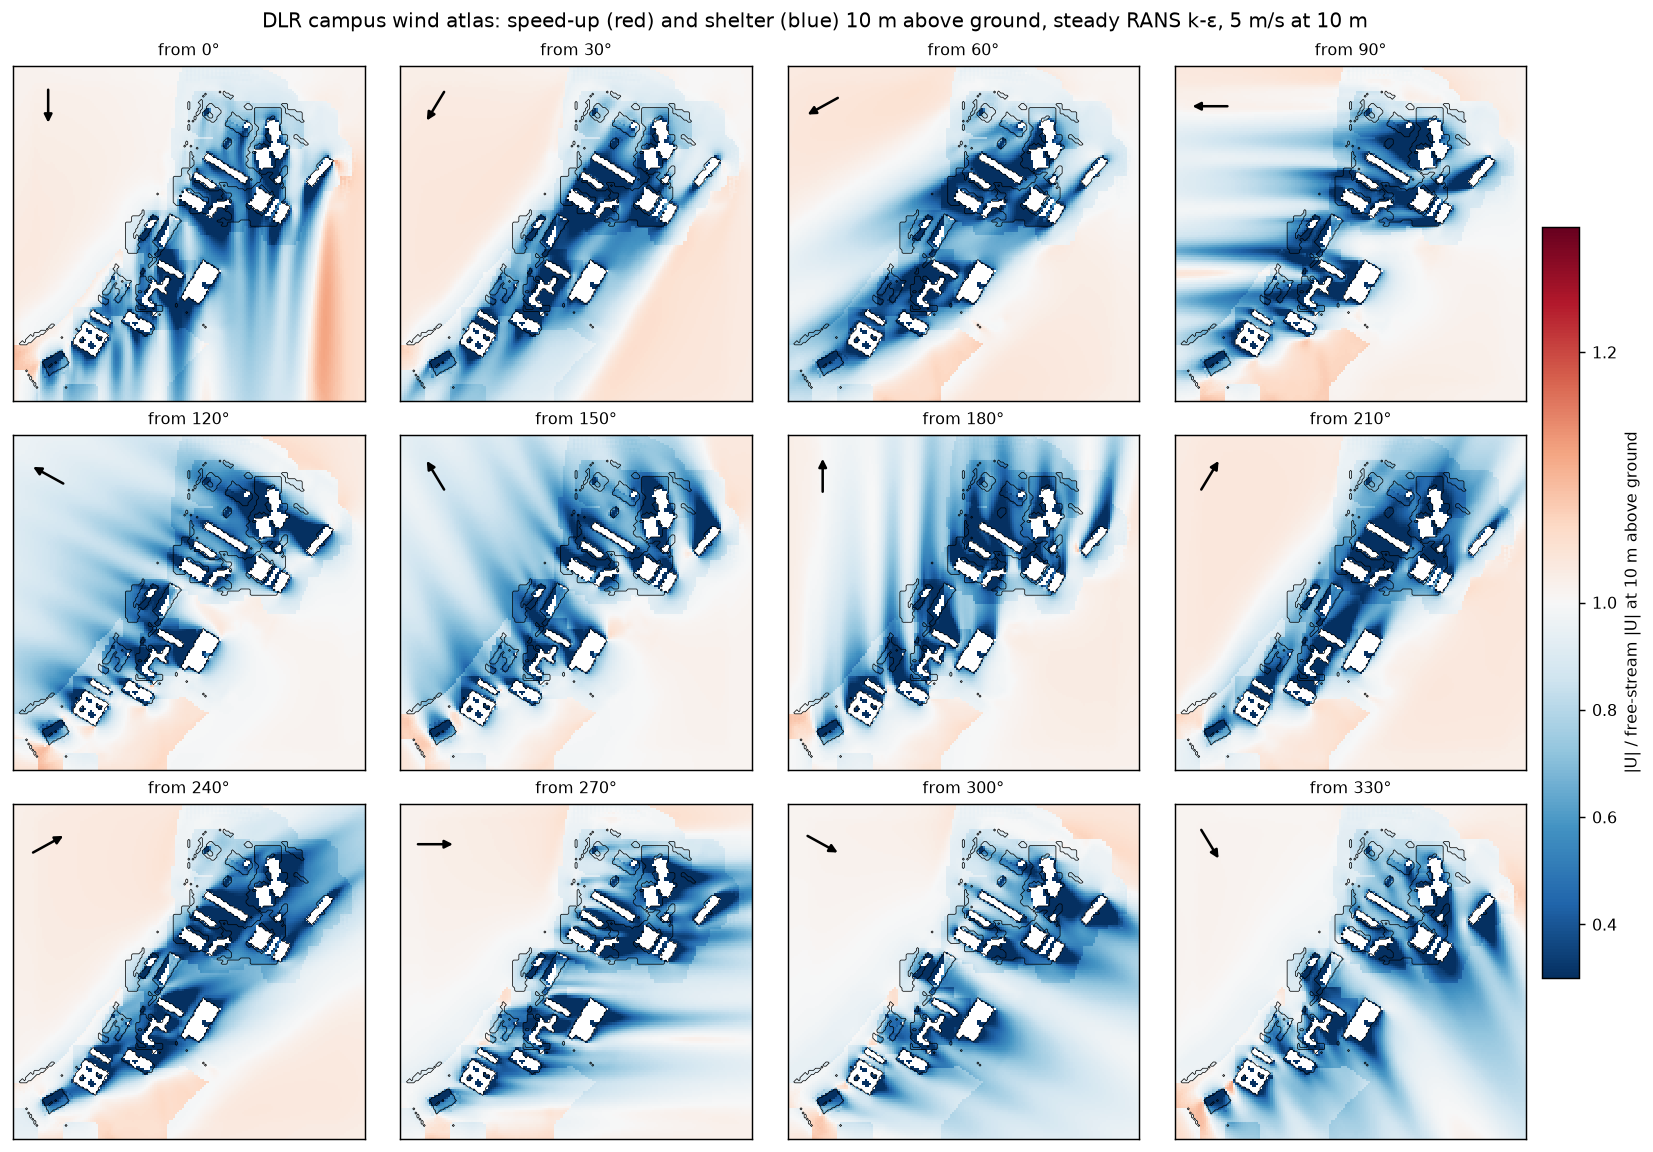
\includegraphics[height=0.80\textheight,keepaspectratio]{atlas_maps_10m.png}
\end{frame}

\begin{frame}{The atlas, 30\,m above ground: wakes fade with height}
\centering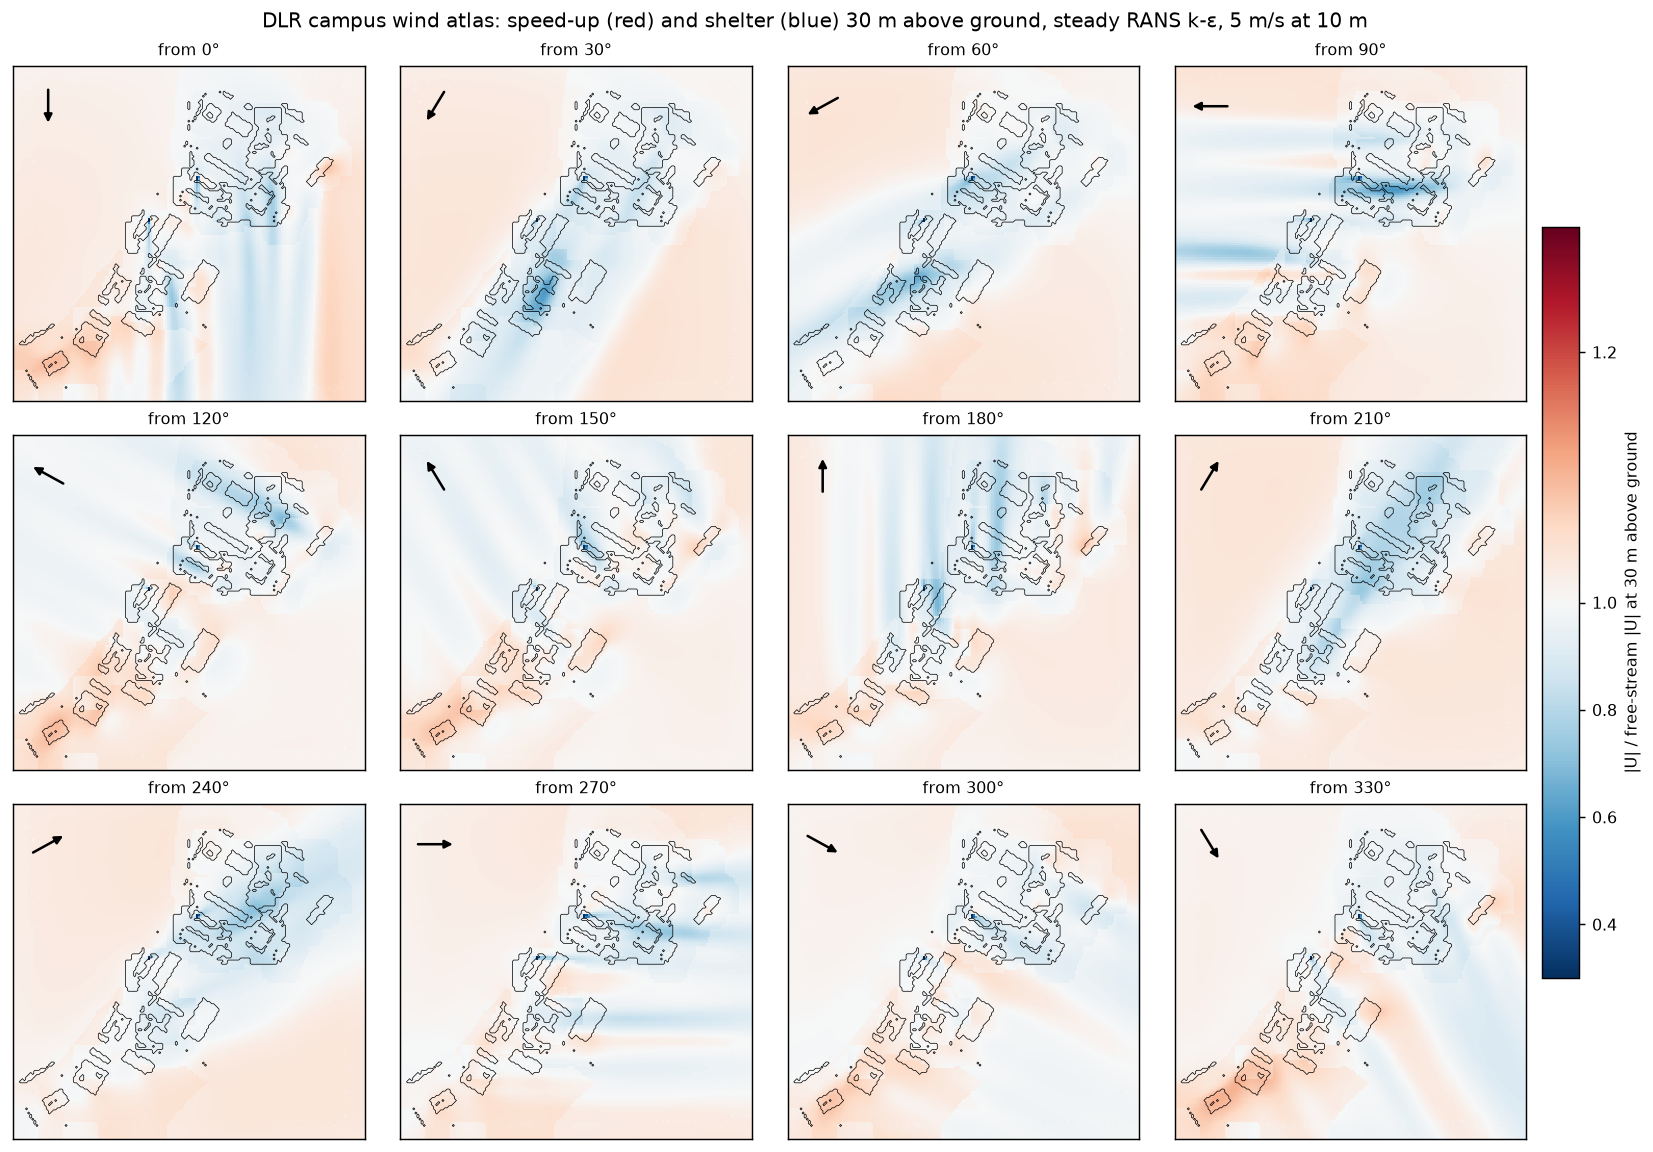
\includegraphics[height=0.80\textheight,keepaspectratio]{atlas_maps_30m.png}
\end{frame}

% ---------------------------------------------------------------------------------------------
\begin{frame}{Can we trust the shortcuts? Speed scaling and direction blending}
\begin{columns}[T]
\begin{column}{0.49\textwidth}\small
\textbf{Speed scaling} (240\,$^\circ$ at 10\,m/s vs.\ $2\times$ the 5\,m/s run):\\
RMS error \ReynoldsRmsTwenty\,\% of $U_\mathrm{ref}$ at 20\,m, \ReynoldsRmsTen\,\% at 10\,m.
\pic{\linewidth}{atlas_reynolds.png}
\end{column}
\begin{column}{0.49\textwidth}\small
\textbf{Direction blending}: hide a solved direction, predict it from its neighbours.\\
\BlendSentence
\pic{\linewidth}{atlas_loo.png}
\end{column}
\end{columns}
\end{frame}

% ---------------------------------------------------------------------------------------------
\begin{frame}{Cost against accuracy: what each wind model buys}
\small
RMS vector error over the campus (air within 60\,m of a building), as a fraction of the 10\,m wind speed:
\medskip

\centering
\begin{tabular}{@{}lrrrrr@{}}
\toprule
Model & Cost per new direction & 10\,m & 20\,m & 40\,m & 60\,m \\
\midrule
Empty-field log-law (no CFD) & 0 & 44.0\,\% & 24.2\,\% & 5.6\,\% & 4.3\,\% \\
Nearest solved run, as is (60$^\circ$ gap) & $\mu$s & 41.7\,\% & 54.8\,\% & 67.9\,\% & 73.3\,\% \\
Nearest solved run, rotated (60$^\circ$ gap) & $\mu$s & 20.0\,\% & 15.8\,\% & 5.1\,\% & 2.6\,\% \\
Linear blend of raw vectors (60$^\circ$ gap) & $\mu$s & 16.5\,\% & 18.1\,\% & 17.9\,\% & 19.0\,\% \\
\textbf{Rotate, then blend} (60$^\circ$ gap) & $\mu$s & 14.1\,\% & 12.0\,\% & 3.7\,\% & 1.6\,\% \\
\textbf{Rotate, then blend} (30$^\circ$, real spacing) & $\mu$s & 7.1\,\% & 7.5\,\% & 2.3\,\% & 0.6\,\% \\
Full CFD for that direction & 25--35 min & 0.0\,\% & 0.0\,\% & 0.0\,\% & 0.0\,\% \\
\bottomrule
\end{tabular}


\medskip
\raggedright\footnotesize
The empty-field log-law is what a planner would assume without any CFD. All errors are against our own RANS model (a model reference, not measured wind), so the ``full CFD'' row is zero by definition. 60$^\circ$ rows: \NLoo{} hidden direction(s); 30$^\circ$ row: 1.
\end{frame}

% ---------------------------------------------------------------------------------------------
\begin{frame}{Drone power and the drag function}
\begin{columns}[T]
\begin{column}{0.47\textwidth}\small
Rotary-wing model of Zeng, Xu \& Zhang (IEEE TWC 2019), the standard one in UAV communications:
\[
P(V)=\underbrace{P_0\!\left(1+\tfrac{3V^2}{U_\mathrm{tip}^2}\right)}_{\text{blade profile}}
+\underbrace{P_i\Big(\sqrt{1+\tfrac{V^4}{4v_0^4}}-\tfrac{V^2}{2v_0^2}\Big)^{1/2}}_{\text{induced (lift)}}
+\underbrace{\tfrac12 d_0\rho sAV^3}_{\text{drag}\,\times\,V}
\]
\vspace{-1em}
\begin{itemize}\setlength{\itemsep}{1pt}
  \item Wind enters through the \textbf{airspeed}: $V=|\mathbf v_g-\mathbf w|$.
  \item Drag force $\mathbf D=-\tfrac12\rho\,(d_0sA)\,|\mathbf v_a|\,\mathbf v_a$.
  \item Climb adds $W\dot z$; descent gets no credit.
  \item Hover \HoverW\,W; cheapest cruise \BestJm\,J/m at \BestSpeed\,m/s (2\,kg reference UAV).
\end{itemize}
\end{column}
\begin{column}{0.51\textwidth}
\centering\pic{\linewidth}{energy_power_breakdown.png}
\end{column}
\end{columns}
\end{frame}

\begin{frame}{Wind changes both the cost per metre and the best speed}
\begin{columns}[T]
\begin{column}{0.58\textwidth}
\centering\pic{\linewidth}{energy_per_metre_wind.png}
\end{column}
\begin{column}{0.4\textwidth}\small
5\,m/s wind, drone free to choose its speed:
\begin{itemize}\setlength{\itemsep}{2pt}
  \item headwind: 11.9\,J/m (+34\,\%), best ground speed 15.8\,m/s;
  \item tailwind: 6.9\,J/m ($-$22\,\%), best ground speed 21.6\,m/s.
\end{itemize}
Into a headwind the drone should fly \emph{faster through the air} (20.8\,m/s airspeed): time in the wind costs hover power.
\end{column}
\end{columns}
\end{frame}

\begin{frame}{Does the battery's nonlinearity change the answer? (Stefano's question)}
\begin{columns}[T]
\begin{column}{0.62\textwidth}
\centering\pic{\linewidth}{energy_battery_losses.png}
\end{column}
\begin{column}{0.36\textwidth}\small
Equivalent-circuit LiPo pack (6S, 5\,Ah, $R_\mathrm{int}$, OCV curve): $I^2R$ losses grow with power.
\begin{itemize}\setlength{\itemsep}{2pt}
  \item Warm pack: losses $\approx$\,2\,\% of the energy; the optimal speed moves by only 0.2\,m/s.
  \item Cold or aged pack at 20\,\% charge: losses up to 8\,\% at cruise, and aggressive power pulses cost 16--19\,\% more cell energy.
\end{itemize}
\textbf{So:} minimising propulsion energy is enough for planning; the battery matters for low-charge, cold or aggressive flight.
\end{column}
\end{columns}
\end{frame}

% ---------------------------------------------------------------------------------------------
\begin{frame}{Planner: shortest path vs.\ minimum-energy path}
\begin{columns}[T]
\begin{column}{0.5\textwidth}\small
\textbf{Graph:} the atlas grid coarsened to 10\,m $\times$ 10\,m $\times$ 5\,m, \PlanNodes{} free nodes from 10 to 100\,m above ground, obstacles inflated by 5\,m, 26 neighbours per node.

\medskip
\textbf{Directed edges:} $c_{ij}\neq c_{ji}$: the same segment costs more upwind than downwind at efficient airspeeds.
\[
c_{ij}=\frac{P\big(|v_g\hat{\mathbf d}_{ij}-\mathbf w_{ij}|\big)}{v_g}\,\ell_{ij}\quad\text{[J]}
\]
\textbf{Solver:} Dijkstra (exact on the graph). Baseline: same graph, cost $=\ell_{ij}$.

\medskip
\textbf{Fair comparison:} both paths re-evaluated in the same wind, sampled every 2\,m.
\end{column}
\begin{column}{0.48\textwidth}
\centering\pic{\linewidth}{\PlanMapFile}
\end{column}
\end{columns}
\end{frame}

\begin{frame}{Planner results: which lever saves energy?}
\centering\small\begin{tabular}{@{}lrr@{}}
\toprule
Lever (climate-weighted, \% of energy) & typical & 8\,m/s \\
\midrule
efficient speed, not wind: 18.3 vs.\ 10\,m/s, still air & 30 & 29 \\
wind-adaptive speed: best per segment vs.\ 18.3\,m/s & 1.2 & 4.7 \\
wind-aware route, both at best speed & 0.7 & 4.6 \\
wind-aware route, fixed 10\,m/s & 0.3 & 2.1 \\
(not a saving: zero on a round trip) energy gap A$\to$B vs.\ B$\to$A & 30 & 62 \\
\bottomrule
\end{tabular}


\medskip
\raggedright\small
\PlanSentence
\end{frame}

\begin{frame}{Planner results by wind direction}
\centering\footnotesize\begin{tabular}{@{}rr rrr rrr@{}}
\toprule
 & & \multicolumn{3}{c}{typical wind (EDMO mean)} & \multicolumn{3}{c}{8\,m/s} \\
\cmidrule(lr){3-5}\cmidrule(l){6-8}
from & reports & $U_{10}$ & 10\,m/s & best speed & 10\,m/s & best speed & p90 \\
 & (\%) & (m/s) & \multicolumn{2}{c}{energy saved (\%)} & \multicolumn{2}{c}{energy saved (\%)} & best \\
\midrule
0$^\circ$ & 3.6 & 3.0 & 0.2 & 0.4 & 1.5 & 4.6 & 14 \\
30$^\circ$ & 7.1 & 3.1 & 0.1 & 0.5 & 2.5 & 5.1 & 13 \\
60$^\circ$ & 8.3 & 3.3 & 0.2 & 0.6 & 3.3 & 5.8 & 15 \\
90$^\circ$ & 6.1 & 2.9 & 0.3 & 0.3 & 2.3 & 4.8 & 13 \\
120$^\circ$ & 3.1 & 2.0 & 0.1 & 0.2 & 0.7 & 2.3 & 7 \\
150$^\circ$ & 6.8 & 2.1 & 0.1 & 0.2 & 0.9 & 2.6 & 9 \\
180$^\circ$ & 8.2 & 2.1 & 0.2 & 0.3 & 1.8 & 4.8 & 14 \\
210$^\circ$ & 15.8 & 3.0 & 0.2 & 0.5 & 2.3 & 5.1 & 13 \\
240$^\circ$ & 22.9 & 5.2 & 0.5 & 1.6 & 2.6 & 5.3 & 13 \\
270$^\circ$ & 10.3 & 4.3 & 0.4 & 0.6 & 1.7 & 4.3 & 13 \\
300$^\circ$ & 4.1 & 3.4 & 0.3 & 0.3 & 0.6 & 2.1 & 9 \\
330$^\circ$ & 3.7 & 3.1 & 0.3 & 0.3 & 0.8 & 2.4 & 10 \\
\bottomrule
\end{tabular}


\medskip
\raggedright\footnotesize
Energy saved by the wind-aware path over the smoothed shortest path (both at 10\,m/s, or both at the best speed per segment). Reports: share of
EDMO 2020--2025 reports per sector. Typical wind: the sector's mean speed.
\end{frame}

% ---------------------------------------------------------------------------------------------
\begin{frame}{Limits, next steps, and questions}
\begin{columns}[T]
\begin{column}{0.48\textwidth}\small
\textbf{Limits}
\begin{itemize}\setlength{\itemsep}{1pt}
  \item Steady RANS, neutral atmosphere: mean wind only, no gusts.
  \item No validation against measured wind (DLR station data pending).
  \item Invented flat terrain outside the original strip.
  \item Planner: steady wind, quasi-steady power, no acceleration or turn costs.
\end{itemize}
\textbf{Next}
\begin{itemize}\setlength{\itemsep}{1pt}
  \item Add turbulence ($\sqrt{k}$) as a risk term; add the RF term.
  \item RL: prototype environment done (reward $=-$energy, exact Dijkstra oracle; a tabular agent reaches the optimum). Next: PPO over the whole wind climate.
  \item Run the same pipeline on the RF group's scenarios.
\end{itemize}
\end{column}
\begin{column}{0.5\textwidth}\small
\textbf{Questions}
\begin{enumerate}\setlength{\itemsep}{2pt}
  \item Which drone should the energy model represent (mass, size)? A real DLR platform?
  \item Fausto's lookup and this atlas: same grid and file format for both scenes?
  \item Flight envelope for the planner: altitude band, clearance, airfield restrictions?
  \item Can we get the DLR weather-station data for a first validation?
\end{enumerate}
\end{column}
\end{columns}
\end{frame}

\end{document}
